\documentclass[12pt,a4paper]{article}
\usepackage{amsmath, amssymb}
\usepackage{geometry}
\usepackage{hyperref}
\usepackage{booktabs}
\usepackage{graphicx}
\usepackage{setspace}
\usepackage{float}
\usepackage{tikz}
\usetikzlibrary{arrows.meta, positioning, shapes.geometric}
\graphicspath{{assets/}}

%title page
\geometry{margin=1in}

\begin{document}
\onehalfspacing

% Title Page
\begin{titlepage}
    \centering
        
    \Huge
    \textbf{Jaypee Institute of Information Technology, Sector - 62, Noida } \\
    \vspace{0.5cm}
    \Large
    \textbf{B.Tech CSE III Semester}\\
    \vspace{1cm}
    % \vspace*{\fill}
        
    \includegraphics[scale=0.2]{jiit_logo}\\
        
    \vspace{1.5cm}
    \Huge
    \textbf{DS Lab PBL Report}\\
    \normalsize
    
        
    \textbf{Terminal Data Structures \& Algorithms Visualizer}\\
    \vspace{1cm}
    
    \Large
    \textbf{Submitted to}\\
    Dr. Dhanalekshmi G\\
    Dr. Anupama Padha\\[1cm]

    \textbf{Submitted by}
    \vspace{0.5cm}
    \\
    \begin{tabular}{lll}
        Harsh Sharma & 2401030232 & B5\\
        Karvy Singh & 2401030234 & B5\\
        Rudra Kumar Singh & 2401030237 & B5\\
    \end{tabular}
    
    \vspace*{\fill}
    \normalsize
\end{titlepage}

%letter of transmittal 
\begin{center}
    \Large\textbf{Letter of Transmittal}
\end{center}
\vspace{1cm}

\noindent
\textbf{Dr. Dhanalekshmi G}\\
\textbf{Dr. Anupama Padha}\\
[0.5em]
Department of Computer Science \& IT\\
[0.5em]

\vspace{1cm}

\noindent
\textbf{Subject:} Submission of Project ``Terminal Data Structures \& Algorithms Visualizer''

\vspace{1cm}

\noindent
Respected Madam/Sir,

\vspace{1em}

\noindent
We are pleased to submit our project titled \textit{``Terminal Data Structures \& Algorithms Visualizer''} as part of the Data Structures Lab Project Based Learning (PBL) component of the B.Tech CSE III Semester curriculum. This report documents the design, implementation, and analysis of a terminal-based interactive visualizer for classical data structures and sorting algorithms implemented in C++.

\vspace{1em}

\noindent
We have endeavoured to cover the complete lifecycle of the project, including problem formulation, system design, algorithmic choices, implementation details, testing, and observations. Special emphasis has been laid on how different data structures (trees, heaps, B-trees, etc.) and algorithms (Quick Sort, Merge Sort) are modelled, visualized, and interacted with in a text-based terminal environment.

\vspace{1em}

\noindent
Thank you for your guidance and the opportunity to work on this project, which significantly strengthened our understanding of data structures, algorithms, and low-level terminal programming in Unix.

\vspace{1em}

\noindent
Sincerely, \\[1em]

\noindent
Harsh Sharma (2401030232)\\
Karvy Singh (2401030234)\\
Rudra Kumar Singh (2401030237)\\

\vspace{1em}

\noindent
Date: \today

\newpage

\tableofcontents

\newpage

\section{Introduction}

Data structures and algorithms form the foundation of computer science. While they are usually studied through diagrams and pseudocode, understanding their \emph{dynamic behaviour}---how nodes move during rotations, how heaps restructure themselves, or how partitioning behaves in quick sort---is much easier with visual aids.

Most available visualizers are graphical and depend on GUI frameworks or web technologies. In this project we explore a different design space: a \textbf{pure terminal-based visualizer} running in a Unix environment, implemented entirely in C++ using raw terminal control and ASCII art. The goal is to provide:

\begin{itemize}
    \item An interactive way to insert, delete, and inspect elements in various tree and heap structures.
    \item A step-by-step execution view for divide-and-conquer sorting algorithms.
    \item A modular architecture where new data structure ``scenes'' can be added easily.
\end{itemize}

The visualizer demonstrates the runtime behaviour of:

\begin{itemize}
    \item Binary Search Tree (BST)
    \item AVL Tree
    \item Red--Black Tree
    \item Max Heap and Min Heap
    \item Binomial Heap and Fibonacci Heap
    \item B-Tree and B+ Tree
    \item Merge Sort and Quick Sort
\end{itemize}

All of these are integrated under a common scene-based framework controlled through a central event loop operating directly on the Unix terminal.

\section{Problem Statement and Objectives}

\subsection{Problem Statement}

Students often struggle to connect the abstract definitions of data structures and algorithms with their actual runtime behaviour. Existing tools are usually GUI-based, browser-based, or language-specific, which may not fit well in a Unix lab context focused on systems programming.

Hence, the problem we address is:

\begin{quote}
    \textbf{To design and implement a modular, extensible, and purely terminal-based data structures and algorithms visualizer in C++, suitable for Unix lab usage, that can demonstrate the real-time behaviour of classical tree structures, heaps, and sorting algorithms.}
\end{quote}

\subsection{Objectives}

\begin{itemize}
    \item Implement a generic scene management framework to host multiple visualizations in a single executable.
    \item Provide interactive insertion and deletion for tree-based data structures and heaps.
    \item Provide step-by-step visualization for Quick Sort and Merge Sort with information about indices and partitions.
    \item Implement a reusable tree rendering engine based on an abstract \texttt{TreeScene} template.
    \item Use only terminal control (no external GUI frameworks) for portability and simplicity.
    \item Ensure the code is readable, modular, and easily extensible for additional data structures.
\end{itemize}


\section{System Design}

\subsection{High-Level Architecture}

The visualizer is designed around three main layers:

\begin{enumerate}
    \item \textbf{Terminal Abstraction Layer}: Low-level interaction with the Unix terminal using raw mode, ANSI escape codes, and input polling (implemented in \texttt{tui.cpp} and \texttt{tui.h}).
    \item \textbf{Scene Management Layer}: Abstract \texttt{Scene} interface representing different screens (menu, tree visualizers, sorting visualizers), and a global event loop in \texttt{main.cpp} that dispatches events to the current scene.
    \item \textbf{Data Structure \& Visualization Layer}: Concrete scenes such as \texttt{AVLImpl} embedded in a \texttt{TreeScene<Impl>}, or dedicated scenes like \texttt{MergeSortScene} and \texttt{QuickSortScene}, which internally maintain algorithm state and render it.
\end{enumerate}

\subsection{Class Diagram for Scene Architecture}

Figure~\ref{fig:class-diagram-scene} shows a simplified class diagram of the scene and visualization framework. The base class \texttt{Scene} is extended by specific scenes such as \texttt{MenuScene}, \texttt{TreeScene<Impl>}, and algorithm scenes.

\begin{figure}[H]
    \centering
    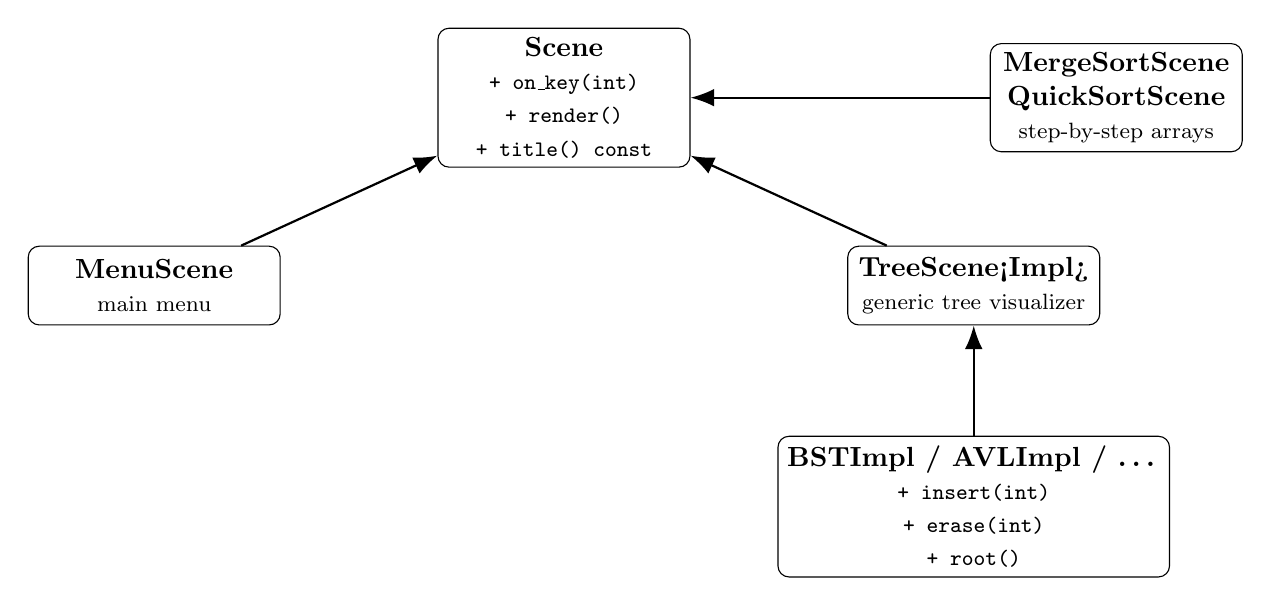
\begin{tikzpicture}[
        class/.style={rectangle, draw, rounded corners, align=center, minimum width=3.2cm, minimum height=1cm},
        arrow/.style={-{Latex[length=3mm]}, thick},
        node distance=1.4cm
    ]
        \node[class] (Scene) {%
            \textbf{Scene}\\
            \footnotesize \texttt{+ on\_key(int)}\\
            \footnotesize \texttt{+ render()}\\
            \footnotesize \texttt{+ title() const}
        };

        \node[class, below left=of Scene, xshift=-1cm] (MenuScene) {%
            \textbf{MenuScene}\\
            \footnotesize main menu
        };

        \node[class, below right=of Scene, xshift=1cm] (TreeScene) {%
            \textbf{TreeScene<Impl>}\\
            \footnotesize generic tree visualizer
        };

        \node[class, below=of TreeScene] (Impl) {%
            \textbf{BSTImpl / AVLImpl / \dots}\\
            \footnotesize \texttt{+ insert(int)}\\
            \footnotesize \texttt{+ erase(int)}\\
            \footnotesize \texttt{+ root()}
        };

        \node[class, right=3.8cm of Scene] (SortScene) {%
            \textbf{MergeSortScene}\\
            \textbf{QuickSortScene}\\
            \footnotesize step-by-step arrays
        };

        \draw[arrow] (MenuScene) -- (Scene);
        \draw[arrow] (TreeScene) -- (Scene);
        \draw[arrow] (SortScene) -- (Scene);
        \draw[arrow] (Impl) -- (TreeScene);
    \end{tikzpicture}
    \caption{Simplified class diagram of the scene and visualization architecture.}
    \label{fig:class-diagram-scene}
\end{figure}

\subsection{Event Loop and Control Flow}

The central event loop is implemented in \texttt{main.cpp}. It:

\begin{enumerate}
    \item Initializes the terminal (\texttt{init()}).
    \item Sets the current scene to the menu scene (\texttt{make\_menu\_scene()}).
    \item Repeatedly:
    \begin{itemize}
        \item Renders the current scene.
        \item Polls for a key press using \texttt{poll\_key()}.
        \item Dispatches the key to \texttt{on\_key()} of the current scene.
        \item Checks the global \texttt{g\_should\_quit} flag.
    \end{itemize}
    \item Deinitializes the terminal (\texttt{deinit()}).
\end{enumerate}

Figure~\ref{fig:event-loop} gives a flowchart of this control flow.

\begin{figure}[H]
    \centering
    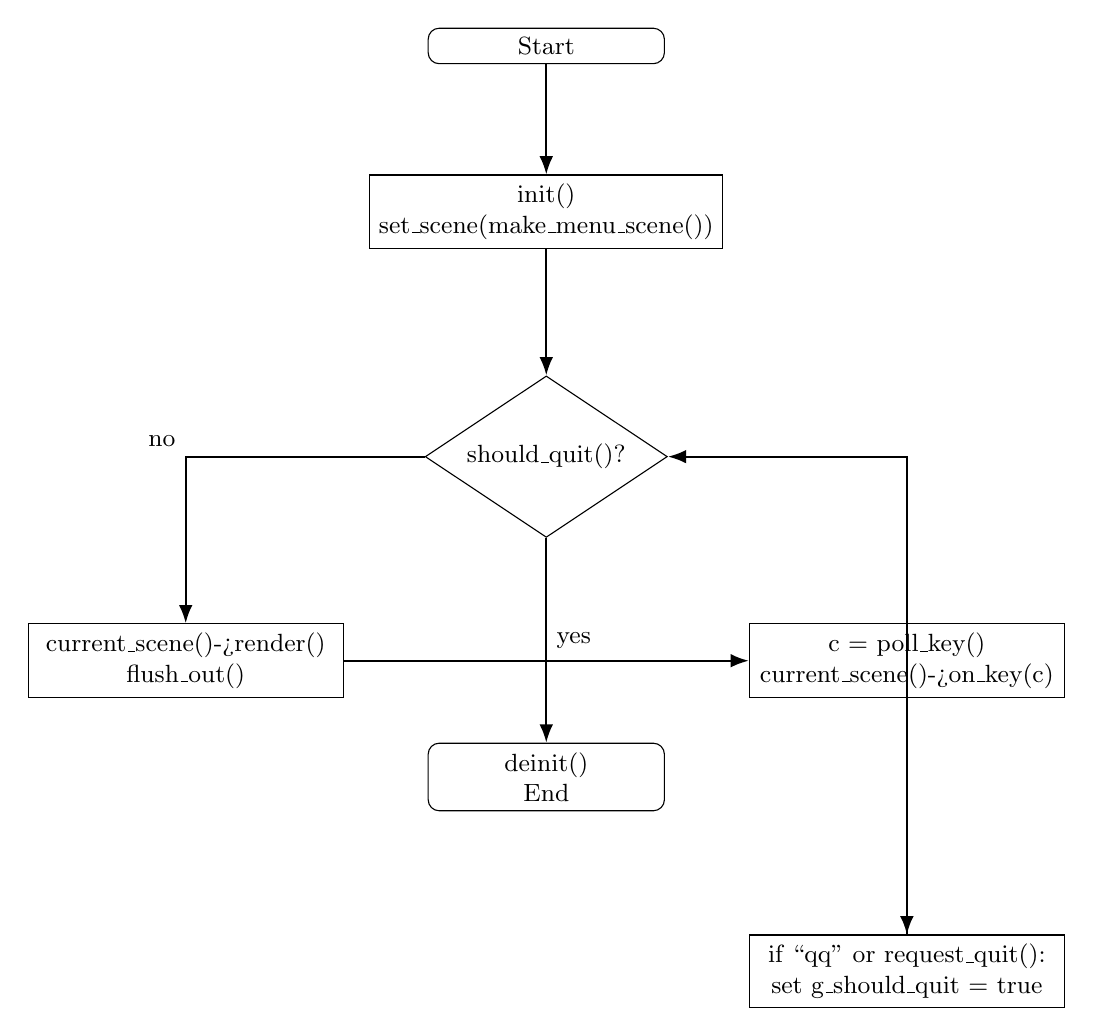
\begin{tikzpicture}[
        node distance=1.4cm,
        >=Latex,
        every node/.style={font=\small},
        startstop/.style={rectangle, rounded corners, draw, align=center, minimum width=3cm},
        process/.style={rectangle, draw, align=center, minimum width=4cm},
        decision/.style={diamond, draw, aspect=1.5, align=center},
        arrow/.style={->, thick}
    ]
        \node[startstop] (start) {Start};
        \node[process, below=of start] (init) {init() \\ set\_scene(make\_menu\_scene())};
        \node[decision, below=of init, yshift=-0.2cm] (quit) {should\_quit()?};
        \node[process, below left=1.6cm and 1.8cm of quit] (render) {current\_scene()->render() \\ flush\_out()};
        \node[process, below right=1.6cm and 1.8cm of quit] (key) {c = poll\_key() \\ current\_scene()->on\_key(c)};
        \node[process, below=3.0cm of key] (updatequit) {if ``qq'' or request\_quit():\\ set g\_should\_quit = true};
        \node[startstop, below=2.6cm of quit] (end) {deinit() \\ End};

        \draw[arrow] (start) -- (init);
        \draw[arrow] (init) -- (quit);

        \draw[arrow] (quit.south) -- node[right]{yes} (end.north);

        \draw[arrow] (quit.west) -| node[above left]{no} (render.north);
        \draw[arrow] (render) -- (key);
        \draw[arrow] (key) -- (updatequit);
        \draw[arrow] (updatequit) |- (quit.east);
    \end{tikzpicture}
    \caption{Event loop and scene control flow in \texttt{main.cpp}.}
    \label{fig:event-loop}
\end{figure}

\subsection{Terminal Rendering Layer}

The file \texttt{tui.cpp} abstracts low-level terminal operations:

\begin{itemize}
    \item Switching the terminal into raw mode using \texttt{termios}.
    \item Clearing the screen and positioning the cursor with ANSI escape sequences.
    \item Reading keys (including special keys like arrows) via \texttt{select()} and non-canonical input.
\end{itemize}

On top of this, drawing helpers in \texttt{draw.cpp} and \texttt{tui.h} provide:

\begin{itemize}
    \item \texttt{frame()}, \texttt{hline()}, \texttt{vline()} for ASCII box drawing.
    \item \texttt{draw\_connector()} for connecting parent and child nodes in tree diagrams.
    \item \texttt{draw\_node\_label()} to render keys as \texttt{[value]}.
\end{itemize}

These are reused by all tree- and heap-based visualizations.

\section{Data Structures and Their Visualization}

\subsection{Common Tree Visualization Framework (\texttt{TreeScene})}

The template \texttt{TreeScene<Impl>} in \texttt{render.h} is a generic scene for any binary tree-like structure. It expects the \texttt{Impl} type to define:

\begin{itemize}
    \item \texttt{using Node = ...;} for the node type.
    \item \texttt{Node *root() const;} returning the root.
    \item \texttt{Node *left(Node*) const;} and \texttt{Node *right(Node*) const;} for child access.
    \item \texttt{void insert(int);} and \texttt{void erase(int);} to modify the structure.
    \item \texttt{void draw\_label(int x, int y, Node *);} for per-node label rendering.
    \item \texttt{vector<int> sample() const;} for sample data.
    \item \texttt{void clear();} to deallocate.
\end{itemize}

\texttt{TreeScene} handles:

\begin{itemize}
    \item Reading numeric input from the user.
    \item Converting \texttt{[Enter]} into an \texttt{insert(int)} call.
    \item Handling \texttt{d} for deletion and \texttt{r} for inserting a sample dataset.
    \item Computing node positions using a recursive layout algorithm so that the left and right subtrees are spaced horizontally.
    \item Drawing connectors and node labels for the entire tree.
\end{itemize}

This framework is reused by:

\begin{itemize}
    \item \texttt{BSTImpl} (Binary Search Tree)
    \item \texttt{AVLImpl} (AVL Tree)
    \item \texttt{RBTImpl} (Red--Black Tree)
    \item \texttt{HeapImpl} (Max Heap)
    \item \texttt{MinHeapImpl} (Min Heap)
\end{itemize}

\subsection{Binary Search Tree (BST)}

The BST is implemented in \texttt{bst/bst.cpp} using a simple \texttt{NodeBST} structure with \texttt{data}, \texttt{left}, and \texttt{right} pointers. The operations are:

\begin{itemize}
    \item \textbf{Insertion}: Recursive insertion (\texttt{insertAVL} reused as a standard BST insert), respecting the BST property:
    \[
        \text{left subtree} < \text{node} < \text{right subtree}.
    \]
    \item \textbf{Deletion}: Handled in \texttt{deleteNodeBST} with three cases:
    \begin{enumerate}
        \item Leaf node.
        \item Node with one child.
        \item Node with two children, where the in-order successor (\texttt{minValueNodeBST}) is used.
    \end{enumerate}
\end{itemize}

The \texttt{BSTImpl} struct plugs this node type into the \texttt{TreeScene} template by providing \texttt{insert}, \texttt{erase}, and \texttt{root}. As the user inserts or deletes values via the terminal, the tree is updated and re-rendered, allowing the user to observe structural changes.

\subsection{AVL Tree}

The AVL tree implementation in \texttt{avl/avl.cpp} extends the BST concept by maintaining height-balanced nodes:

\begin{itemize}
    \item Each node \texttt{NodeAVL} stores its height.
    \item The \texttt{balance(NodeAVL*)} function computes the balance factor as the difference between left and right subtree heights.
    \item After each insertion or deletion, the node heights are updated and \texttt{balanceNodeAVL} applies:
    \begin{itemize}
        \item Left rotation
        \item Right rotation
        \item Left-Right rotation
        \item Right-Left rotation
    \end{itemize}
\end{itemize}

The visualizer shows the effect of rotations in real-time. Inserting a skewed sequence such as \texttt{10, 20, 30} lets the user see the tree self-balancing into a more compact shape.

\subsection{Red--Black Tree}

The Red--Black Tree is implemented in \texttt{rb/rbt.cpp} using \texttt{NodeRBT} which stores:

\begin{itemize}
    \item \texttt{data}
    \item Pointers to \texttt{parent}, \texttt{left}, \texttt{right}
    \item \texttt{color} field ('R' or 'B')
\end{itemize}

Key operations and invariants:

\begin{itemize}
    \item New nodes are initially inserted as red.
    \item The \texttt{insertfix} function:
    \begin{itemize}
        \item Recolors the parent and uncle when both are red.
        \item Performs rotations (left or right) around the grandparent to fix double-red violations.
        \item Ensures the root is always black.
    \end{itemize}
    \item The \texttt{draw\_label} method renders nodes as \texttt{[keyR]} or \texttt{[keyB]}, with 'R' shown in red using ANSI color codes.
\end{itemize}

This allows students to not only see the structure of the tree, but also how colors change to maintain the Red--Black properties.

\subsection{Max Heap}

The max heap implementation in \texttt{max\_heaps/max\_heaps.cpp} uses a \texttt{vector<int>} to store heap elements. The key functions are:

\begin{itemize}
    \item \texttt{heapifyup(i)} to bubble an inserted element upwards while the parent is smaller.
    \item \texttt{heapifydown(i)} to restore the heap after extraction or key modification.
    \item \texttt{insert(int val)} and \texttt{extractmax()}.
\end{itemize}

For visualization, indices in the array are mapped to nodes via a secondary \texttt{nodes} vector of small \texttt{Node} structs that just store the index. The \texttt{root()}, \texttt{left()}, and \texttt{right()} methods adapt this to the tree visualization engine, displaying the heap as a binary tree.

\subsection{Min Heap}

The min heap (\texttt{min\_heaps/min\_heap.cpp}) mirrors the max heap but maintains the minimum element at the root:

\begin{itemize}
    \item \texttt{getmin()} retrieves \texttt{heap[0]}.
    \item Insertion uses \texttt{heapifyup} with the comparison reversed.
    \item Extraction uses \texttt{heapifydown} to restore the min-heap property.
\end{itemize}

Like the max heap, it reuses the \texttt{TreeScene} rendering to show the implicit array as a binary tree.

\subsection{Binomial Heap}

The binomial heap is implemented in \texttt{bin\_heaps/bin\_heaps.cpp} with a \texttt{Node} structure supporting:

\begin{itemize}
    \item \texttt{key}, \texttt{degree}
    \item Pointers to \texttt{parent}, \texttt{child}, and \texttt{sibling}
\end{itemize}

Key operations:

\begin{itemize}
    \item \texttt{mergeRootLists} to merge two root lists sorted by degree.
    \item \texttt{unionHeaps} to link trees of equal degree and maintain the binomial heap invariants.
    \item \texttt{extractMin} which finds the minimum key in the root list, removes the corresponding tree, reverses its children, and unions them back.
\end{itemize}

The visualization uses a custom \texttt{BinomialHeapScene} which:

\begin{itemize}
    \item Draws the roots side-by-side.
    \item Recursively draws children to show the structure of individual binomial trees.
\end{itemize}

\subsection{Fibonacci Heap}

The Fibonacci heap implementation in \texttt{fib\_heaps/fib\_heaps.cpp} uses circular doubly linked lists and lazy consolidation:

\begin{itemize}
    \item Nodes (\texttt{FibNode}) maintain \texttt{key}, \texttt{degree}, \texttt{mark}, parent and child pointers, and circular left/right pointers.
    \item \texttt{insert} adds a node to the root list and updates the global minimum pointer.
    \item \texttt{extractMin}:
    \begin{itemize}
        \item Moves the extracted node's children to the root list.
        \item Calls \texttt{consolidate()} to merge roots of equal degree by linking trees.
    \end{itemize}
\end{itemize}

The visualizer shows each root tree as a separate subtree and allows the user to observe how trees of equal degree coalesce after repeated extractions.

\subsection{B-Tree}

The B-Tree in \texttt{btree/btree.cpp} is parameterized by a minimum degree \texttt{t}. Each node stores multiple keys and child pointers:

\begin{itemize}
    \item Insertion follows the standard B-Tree algorithm:
    \begin{itemize}
        \item Split full children using \texttt{split\_child}.
        \item Insert into non-full nodes (\texttt{insert\_non\_full}).
    \end{itemize}
    \item The \texttt{BTreeScene} stores a list of elements and reconstructs the tree after deletions.
\end{itemize}

Visualization is multi-key: each node is drawn as a box \texttt{[k\_1|k\_2|\dots]} and children are connected beneath. This helps understand how B-Trees maintain balance and high fan-out.

\subsection{B+ Tree}

The B+ Tree in \texttt{bptree/bptree.cpp} extends B-Trees by keeping all data in leaf nodes and linking leaves at the bottom level:

\begin{itemize}
    \item Internal nodes guide the search and store separator keys.
    \item Leaf nodes store actual keys and maintain a linked list via the \texttt{next} pointer.
    \item \texttt{split\_child} handles splitting both leaf and internal nodes differently.
\end{itemize}

The \texttt{BPlusTreeScene}:

\begin{itemize}
    \item Draws internal nodes similarly to B-Trees.
    \item Records the positions of leaves and then draws horizontal arrows between them to illustrate the leaf-level linked list used for range queries.
\end{itemize}

\section{Sorting Algorithms}

\subsection{Quick Sort Visualization}

\texttt{quicksort/quicksort.cpp} implements \texttt{QuickSortScene}, which allows the user to:

\begin{itemize}
    \item Enter integers interactively.
    \item Press \texttt{s} to compute a sequence of steps.
    \item Use \texttt{n} and \texttt{p} to move forward and backward through the recorded steps.
\end{itemize}

The key idea is an instrumented version of quick sort:

\begin{itemize}
    \item Each time the algorithm scans or swaps elements in the partition procedure, it calls \texttt{record\_step}.
    \item A \texttt{Step} struct stores:
    \begin{itemize}
        \item The array snapshot.
        \item \texttt{low}, \texttt{high}, and pivot index.
        \item Scan indices \texttt{i} and \texttt{j}.
        \item A textual description (\texttt{info}) such as ``scan'', ``swap'', or ``pivot placed''.
    \end{itemize}
    \item The \texttt{render()} method draws the current array and overlays index information.
\end{itemize}

This helps visualize the partitioning process and how sub-arrays are recursively sorted.

\subsection{Merge Sort Visualization}

Similarly, \texttt{mergesort/mergesort.cpp} defines \texttt{MergeSortScene}:

\begin{itemize}
    \item Users type numbers and press \texttt{s} to start the sort.
    \item The instrumented merge function records the array after each write back to the main array.
    \item A \texttt{Step} struct stores \texttt{low}, \texttt{mid}, and \texttt{high} indices, along with the array snapshot and an \texttt{info} string.
\end{itemize}

The visualizer shows how two halves are merged repeatedly, reinforcing the concept of divide-and-conquer and stable merging.

\section{User Interaction and Menu Navigation}

\subsection{Menu Scene}

The \texttt{MenuScene} in \texttt{menu\_scene.cpp} lists all available visualizations:

\begin{itemize}
    \item BST
    \item AVL Tree
    \item Red--Black Tree
    \item Max Heap
    \item Min Heap
    \item Binomial Heap
    \item Fibonacci Heap
    \item B-Tree
    \item B+ Tree
    \item Merge Sort
    \item Quick Sort
    \item Quit
\end{itemize}

The user navigates using:

\begin{itemize}
    \item Up/Down arrow keys to move the selection.
    \item \texttt{Enter} or Right arrow to activate the selected scene.
    \item \texttt{q q} sequence to quit from anywhere.
\end{itemize}

\subsection{Key Bindings Inside Visualizers}

Most scenes share common key bindings:

\begin{itemize}
    \item Digit keys (\texttt{0--9}): type into the input buffer.
    \item \texttt{Enter}: convert buffer to number and insert into the current structure.
    \item \texttt{d}: delete the value currently in the buffer (where supported).
    \item \texttt{r}: insert a sample dataset.
    \item \texttt{c}: clear the current data structure or array.
    \item \texttt{b} or \texttt{Esc}: return to the main menu.
    \item \texttt{q q}: exit the program.
\end{itemize}

Sorting scenes additionally use:

\begin{itemize}
    \item \texttt{s}: compute the full set of algorithm steps.
    \item \texttt{n}/\texttt{p}: navigate through recorded steps.
\end{itemize}

Heaps and priority structures may provide extra keys such as \texttt{x} for ``extract minimum'' in the Fibonacci heap scene.

\section{Time Complexity Summary}

Table~\ref{tab:complexity} summarizes the time complexity of the supported data structures and algorithms.

\begin{table}[H]
    \centering
    \begin{tabular}{@{}llll@{}}
        \toprule
        \textbf{Structure / Algorithm} & \textbf{Operation} & \textbf{Average} & \textbf{Worst Case} \\
        \midrule
        BST           & Search/Insert/Delete   & $O(\log n)$      & $O(n)$ \\
        AVL Tree      & Search/Insert/Delete   & $O(\log n)$      & $O(\log n)$ \\
        Red--Black Tree & Search/Insert/Delete & $O(\log n)$      & $O(\log n)$ \\
        Max/Min Heap  & Insert / Extract top   & $O(\log n)$      & $O(\log n)$ \\
        Binomial Heap & Insert / Union / Extract min & $O(\log n)$ & $O(\log n)$ \\
        Fibonacci Heap & Insert                & $O(1)$           & $O(1)$ \\
                      & Extract min           & $O(\log n)$      & $O(\log n)$ \\
        B-Tree/B+ Tree & Search/Insert/Delete & $O(\log n)$      & $O(\log n)$ \\
        Merge Sort    & Sorting               & $O(n \log n)$    & $O(n \log n)$ \\
        Quick Sort    & Sorting               & $O(n \log n)$    & $O(n^2)$ \\
        \bottomrule
    \end{tabular}
    \caption{Time complexity overview of implemented data structures and algorithms.}
    \label{tab:complexity}
\end{table}

\newpage
\section{Screenshots}

\subsection{Main Menu}

\begin{figure}[H]
    \centering
    \fbox{\includegraphics[width=0.9\textwidth]{menu_scene}}
    \caption{Main menu of the Terminal Data Structures \& Algorithms Visualizer (placeholder).}
    \label{fig:menu-scene}
\end{figure}

\subsection{AVL Tree Visualization}

\begin{figure}[H]
    \centering
    \fbox{\includegraphics[width=0.9\textwidth]{avl_scene}}
    \caption{AVL tree after multiple insertions demonstrating rotations (placeholder).}
    \label{fig:avl-scene}
\end{figure}

\subsection{Red--Black Tree Visualization}

\begin{figure}[H]
    \centering
    \fbox{\includegraphics[width=0.9\textwidth]{rbt_scene}}
    \caption{Red--Black tree with node colors indicating balancing (placeholder).}
    \label{fig:rbt-scene}
\end{figure}

\subsection{Quick Sort Step-by-Step Visualization}

\begin{figure}[H]
    \centering
    \fbox{\includegraphics[width=0.9\textwidth]{quicksort_scene}}
    \caption{Quick sort scene showing pivot and partition indices (placeholder).}
    \label{fig:quicksort-scene}
\end{figure}


\subsection{Future Enhancements}

Possible extensions include:

\begin{itemize}
    \item Adding more algorithms such as Dijkstra's shortest path, BFS/DFS visualizations, and hash tables.
    \item Supporting loading inputs from files and saving sessions.
    \item Adding simple profiling information (number of comparisons/rotations/swaps) alongside the visualization.
    \item Porting the same architecture to a GUI or web-based frontend while reusing the core data structure implementations.
\end{itemize}

\section*{References}

\begin{itemize}
    \item Course Material
    \item Thomas H. Cormen, Charles E. Leiserson, Ronald L. Rivest, Clifford Stein, \textit{Introduction to Algorithms}, MIT Press.
    \item Mark Allen Weiss, \textit{Data Structures and Algorithm Analysis in C++}.
\end{itemize}

\appendix

\end{document}
